\chapter{Tutorial on 5G Communication System}
\label{chapter2}
The rapid advancement in the wireless communications shows the huge success in the wireless communication system. The advancement started with second generation (2G) system's debut in 1991 which were commercially launched on the GSM standard in Finland by Radiolinja. 2G systems were significantly more spectrally efficient compared to their predecessors and 2G also introduced the data services for mobile starting with SMS text messages, picture messages and multimedia messages (MMS). From 2G we migrated to 3G system which were first launched in 2001 and had fast mobile internet access. 3G also introduced video calls and mobile TV and was able to provide information transfer speed of at least 2 Mbit/s. The 4G wireless systems were designed to be fully based on IP telephony where all the voice communications and multimedia sessions are delivered over Internet protocol (IP) networks~\cite{4561570}. 4G systems use orthogonal frequency division multiplexing (OFDM), multiple-input multiple-output (MIMO), and link adaptation technologies for a long term evolution (LTE) radio interface. 4G wireless networks can support data rates of up to 1 Gb/s for low mobility and up to 100 Mb/s for high mobility scenarios. The next evolution in wireless mobile communications is the fifth generation (5G) which is expected to be deployed by 2020.

Due to a sharp increase in number of wireless mobile devices and the shortage of the wireless spectrum, researchers have started to investigate 5G wireless technologies. It is expected that the 5G network will achieve 1000 times the system capacity, 10 times the spectral efficiency, energy efficiency, data rate and 25 times the average cell throughput. This translates to a peak data rate of 10 Gb/s for low mobility and peak data rate of 1 Gb/s for high mobility scenarios. The table~\ref{tableG} below shows the comparison between 2G, 3G, 4G and 5G cellular communication system. 
\begin{table}[!ht]
\centering
\caption{Cellular Technologies Comparison between different generations of deployed digital cellular networks. Data rates, standard and implementation technology is compared for the 2G, 3G, 4G and 5G}
\begin{tabular}{| c | c | c | c | c |}
\hline
\textbf{Technology} & \textbf{2G} & \textbf{3G} & \textbf{4G} & \textbf{5G} \\
\hline
Deployment & 1980/1999 & 1990/2002 & 2000/2010 & 2010/2022 \\
\hline
Data Rates & 14.4 -- 64 kbps & 2 Mbps & 200 Mbps -- 1 Gbps (low mobility) & 10 Gbps and higher (low mobility) \\
\hline
Standard & TDMA, CDMA, GSM & WCDMA, CDMA-2000 & Unified Long Term Evolution (LTE) standard & In-progress \\
\hline
\end{tabular}
\end{table}





\section{5G Cellular Architecture}





To address the above challenges and meet the 5G system requirements, we need a dramatic change in the design of cellular architecture. We know that wireless users stay indoors for about 80 percent of time, while only stay ourdoors about 20 percent of the time [8]. The current conventional cellular architecture normally uses an outdoor BS in the middle of a cell communi- cating with mobile users, no matter whether they stay indoors or outdoors. For indoor users com- municating with the outdoor BS, the signals have to go through building walls, and this causes very high penetration loss, which significantly dam- ages the data rate, spectral efficiency, and ener- gy efficiency of wireless transmissions. One of the key ideas of designing the 5G cel- lular architecture is to separate outdoor and indoor scenarios so that penetration loss through building walls can somehow be avoided. This will be assisted by distributed antenna system (DAS) and massive MIMO technology [9], where geo- graphically distributed antenna arrays with tens or hundreds of antenna elements are deployed. While most current MIMO systems utilize two to four antennas, the goal of massive MIMO systems is to exploit the potentially large capacity gains that would arise in larger arrays of anten- nas. Outdoor BSs will be equipped with large antenna arrays with some antenna elements (also large antenna arrays) distributed around the cell and connected to the BS via optical fibers, bene- fiting from both DAS and massive MIMO tech- nologies. Outdoor mobile users are normally equipped with limited numbers of antenna ele- ments, but they can collaborate with each other to form a virtual large antenna array, which together with BS antenna arrays will construct virtual massive MIMO links. Large antenna arrays will also be installed outside of every building to communicate with outdoor BSs or distributed antenna elements of BSs, possibly with line of sight (LoS) components. Large anten- na arrays have cables connected to the wireless access points inside the building communicating with indoor users. This will certainly increase the infrastructure cost in the short term while signifi- cantly improving the cell average throughput, spectral efficiency, energy efficiency, and data rate of the cellular system in the long run. Using such a cellular architecture, as indoor users only need to communicate with indoor wireless access points (not outdoor BSs) with large antenna arrays installed outside build- ings, many technologies can be utilized that are suitable for short-range communications with high data rates. Some examples include WiFi, femtocell, ultra wideband (UWB), mm-wave communications (3–300 GHz) [7], and visible light communications (VLC) (400–490 THz) [10]. It is worth mentioning that mm-wave and VLC technologies use higher frequencies not traditionally used for cellular communications. These high-frequency waves do not penetrate solid materials very well and can readily be absorbed or scattered by gases, rain, and foliage. Therefore, it is hard to use these waves for outdoor and long distance applications. However, with large bandwidths available, mm- wave and VLC technologies can greatly increase the transmission data rate for indoor scenarios. To solve the spectrum scarcity prob- lem, besides finding new spectrum not tradi- tionally used for wireless services (e.g., mm-wave communications and VLC), we can also try to improve the spectrum utilization of existing radio spectra, for example, via cogni- tive radio (CR) networks [11].
The 5G cellular architecture should also be a heterogeneous one, with macrocells, microcells, small cells, and relays. To accommodate high- mobility users such as users in vehicles and high- speed trains, we have proposed the mobile femtocell (MFemtocell) concept [12], which combines the concepts of mobile relay and fem- tocell. MFemtocells are located inside vehicles to communicate with users within the vehicle, while large antenna arrays are located outside the vehicle to communicate with outdoor BSs. An MFemtocell and its associated users are all viewed as a single unit to the BS. From the user point of view, an MFemtocell is seen as a regu- lar BS. This is very similar to the above idea of separating indoor (inside the vehicle) and out- door scenarios. It has been shown in [12] that users using MFemtocells can enjoy high-data-rate services with reduced signaling overhead. The above proposed 5G heterogeneous cellular architecture is illustrated in Fig. 1.



\begin{figure}
\centering
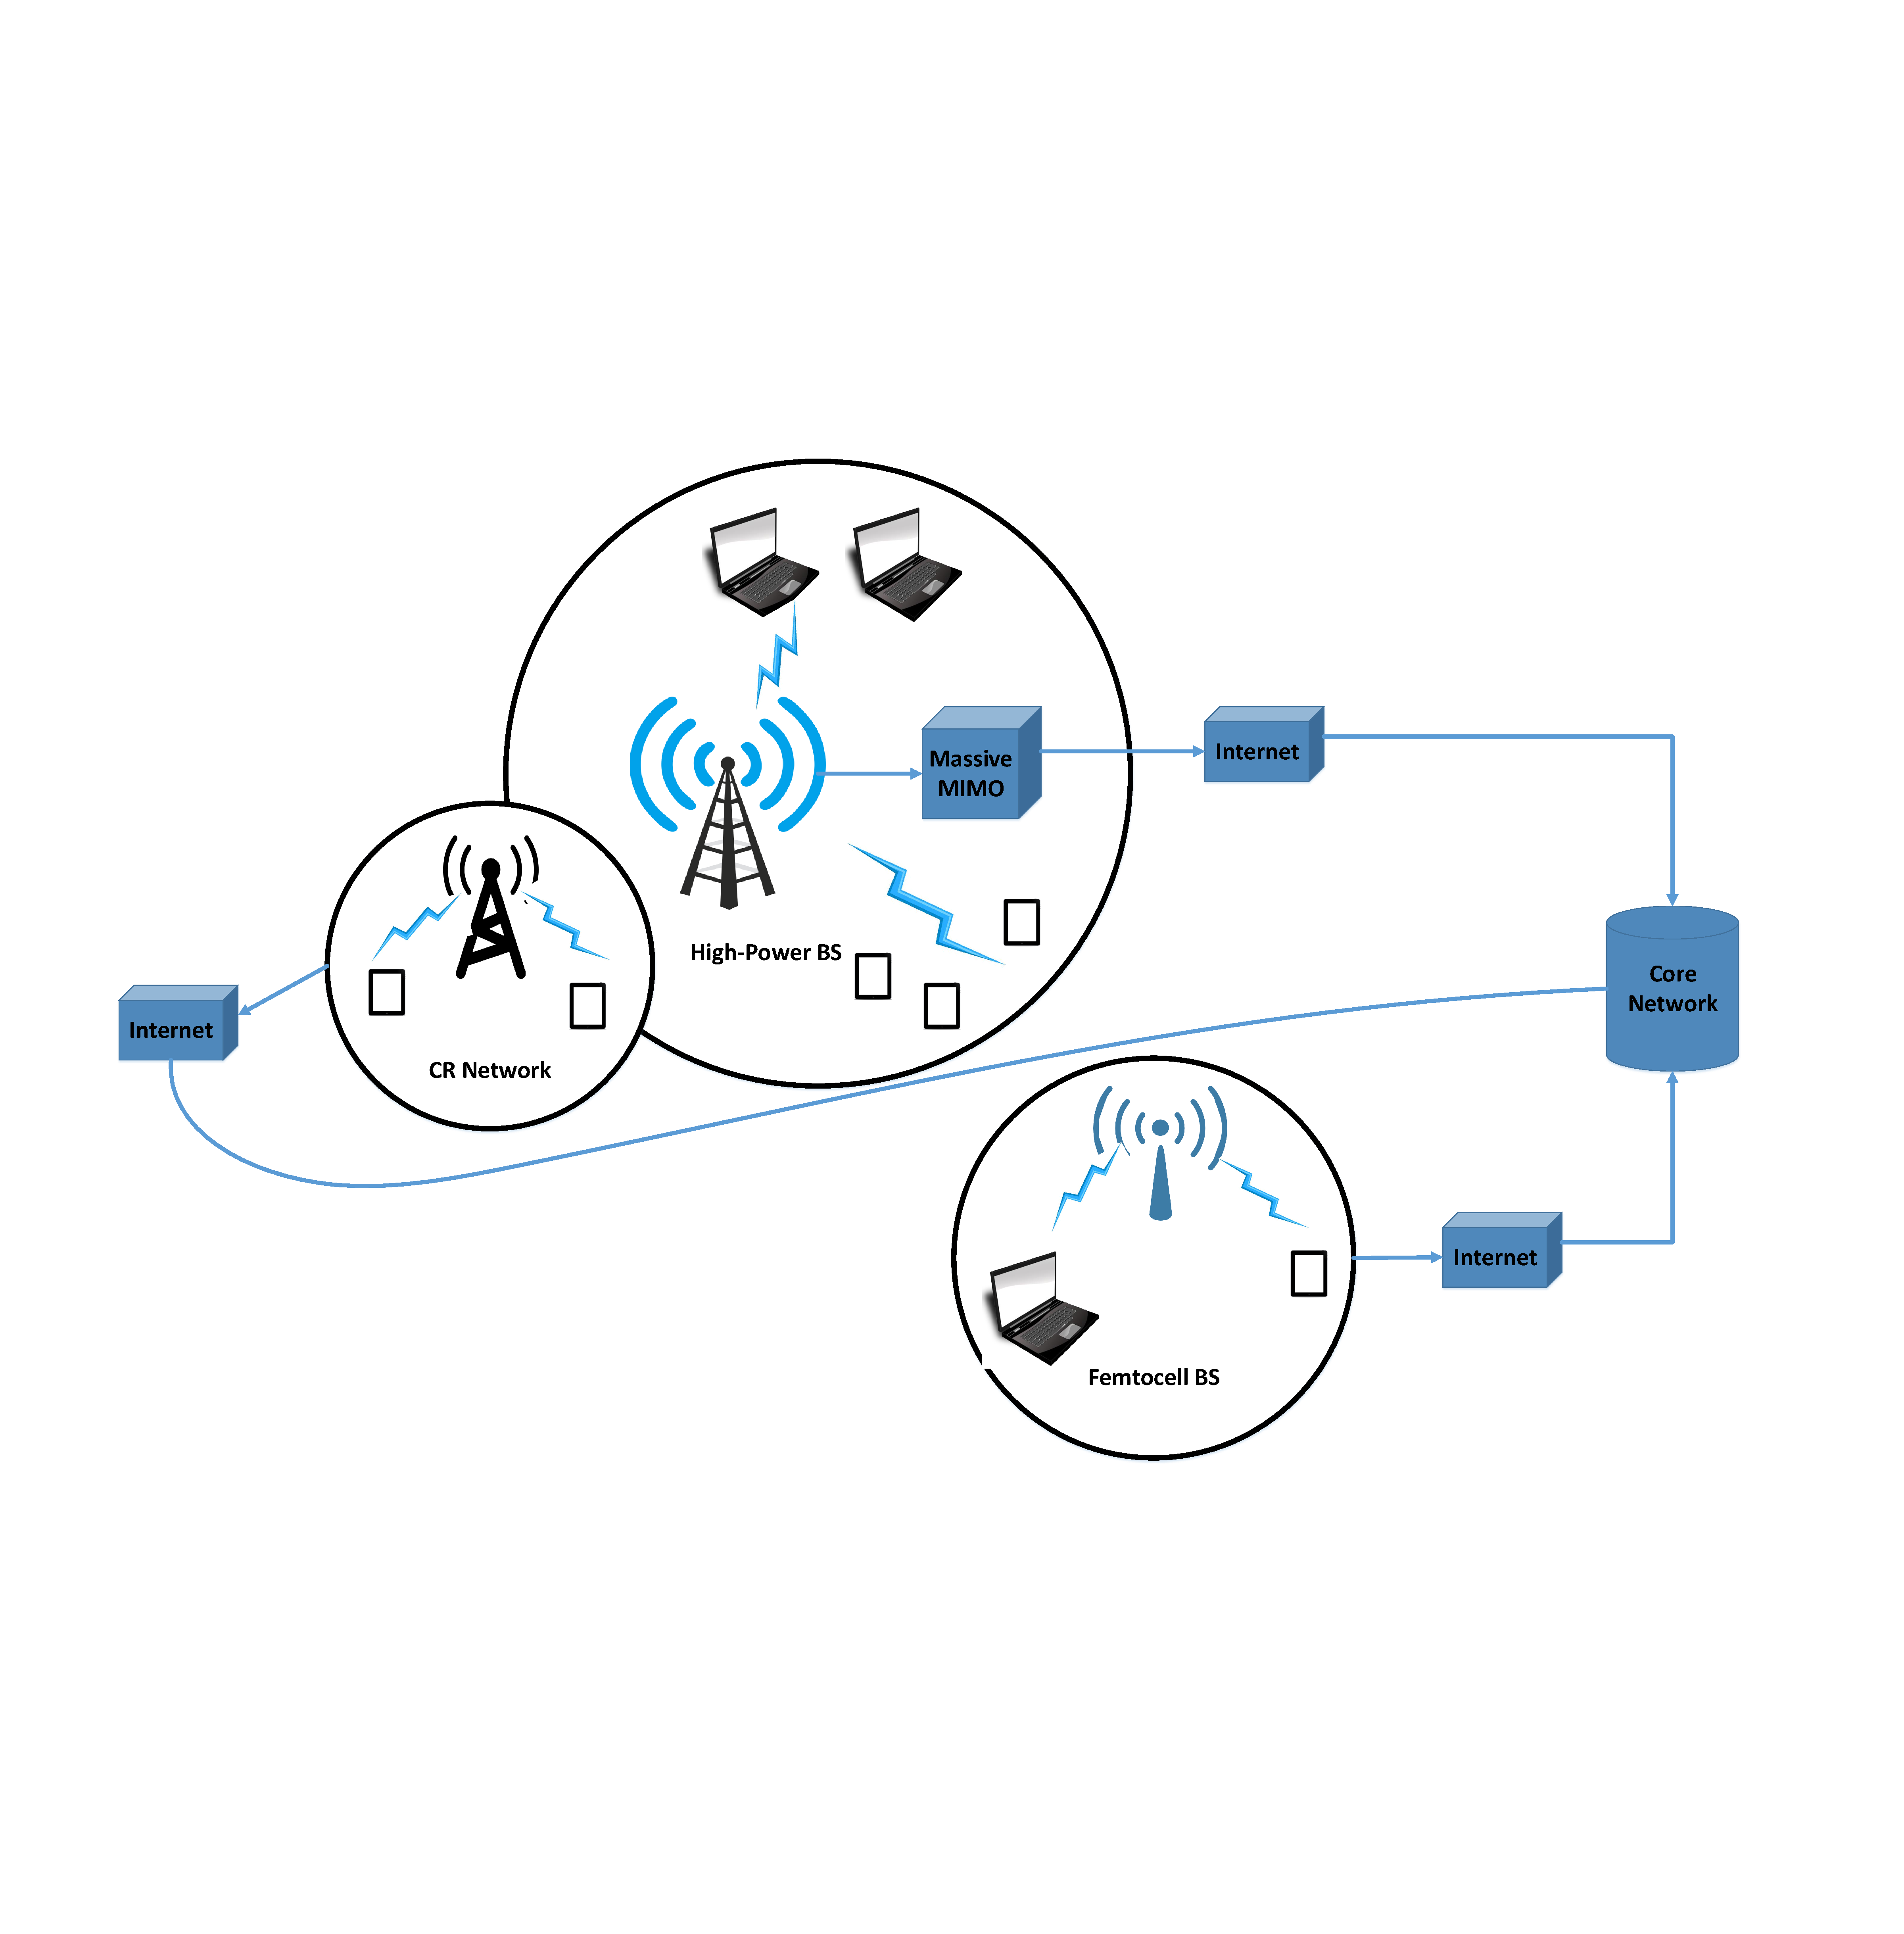
\includegraphics[width=0.75\textwidth,keepaspectratio]{images/Gill/5G/5gsystemarch.eps}
\caption{5G Architecture}
\end{figure}

\section{Key Features of 5G System}
\subsection{Massive MIMO}
\subsection{Machine-to-Machine (M2M) Communication}
\subsection{Internet of Things (IoT)}

\section{5G using Millimeter Wave (mmWave)}

\section{5G in Vehicular Communication}

\section{Current Challenges}

\section{Summary}
This chapter outlined and examined the topics of jamming and anti-jamming techniques, and provided a foundation in communication system theory and advanced equalizer design.  Secondly it setup an understanding of Software-Defined Radio, the power of such an architecture, and examples of implementations and existing software for future designs.  Next, this thesis will consider a new anti-jamming technique and design an implementation of such a system.  After the implementation is investigated, the result of specific experiments on such an implementation will be analyzed.\\
